%% This file was auto-generated by IPython.
%% Conversion from the original notebook file:
%%
\documentclass[11pt,english]{article}

%% This is the automatic preamble used by IPython.  Note that it does *not*
%% include a documentclass declaration, that is added at runtime to the overall
%% document.

\usepackage{amsmath}
\usepackage{amssymb}
\usepackage{graphicx}
\usepackage{grffile}
\usepackage{ucs}
\usepackage[utf8x]{inputenc}
\usepackage{float}

% Scale down larger images
\usepackage[export]{adjustbox}

%fancy verbatim
\usepackage{fancyvrb}
% needed for markdown enumerations to work
\usepackage{enumerate}

% Slightly bigger margins than the latex defaults
\usepackage{geometry}
\geometry{verbose,tmargin=3cm,bmargin=3cm,lmargin=2.5cm,rmargin=2.5cm}

% Define a few colors for use in code, links and cell shading
\usepackage{color}
\definecolor{orange}{cmyk}{0,0.4,0.8,0.2}
\definecolor{darkorange}{rgb}{.71,0.21,0.01}
\definecolor{darkgreen}{rgb}{.12,.54,.11}
\definecolor{myteal}{rgb}{.26, .44, .56}
\definecolor{gray}{gray}{0.45}
\definecolor{lightgray}{gray}{.95}
\definecolor{mediumgray}{gray}{.8}
\definecolor{inputbackground}{rgb}{.95, .95, .85}
\definecolor{outputbackground}{rgb}{.95, .95, .95}
\definecolor{traceback}{rgb}{1, .95, .95}

% new ansi colors
\definecolor{brown}{rgb}{0.54,0.27,0.07}
\definecolor{purple}{rgb}{0.5,0.0,0.5}
\definecolor{darkgray}{gray}{0.25}
\definecolor{lightred}{rgb}{1.0,0.39,0.28}
\definecolor{lightgreen}{rgb}{0.48,0.99,0.0}
\definecolor{lightblue}{rgb}{0.53,0.81,0.92}
\definecolor{lightpurple}{rgb}{0.87,0.63,0.87}
\definecolor{lightcyan}{rgb}{0.5,1.0,0.83}

% Framed environments for code cells (inputs, outputs, errors, ...).  The
% various uses of \unskip (or not) at the end were fine-tuned by hand, so don't
% randomly change them unless you're sure of the effect it will have.
\usepackage{framed}

% remove extraneous vertical space in boxes
\setlength\fboxsep{0pt}

% codecell is the whole input+output set of blocks that a Code cell can
% generate.

% TODO: unfortunately, it seems that using a framed codecell environment breaks
% the ability of the frames inside of it to be broken across pages.  This
% causes at least the problem of having lots of empty space at the bottom of
% pages as new frames are moved to the next page, and if a single frame is too
% long to fit on a page, will completely stop latex from compiling the
% document.  So unless we figure out a solution to this, we'll have to instead
% leave the codecell env. as empty.  I'm keeping the original codecell
% definition here (a thin vertical bar) for reference, in case we find a
% solution to the page break issue.

%% \newenvironment{codecell}{%
%%     \def\FrameCommand{\color{mediumgray} \vrule width 1pt \hspace{5pt}}%
%%    \MakeFramed{\vspace{-0.5em}}}
%%  {\unskip\endMakeFramed}

% For now, make this a no-op...
\newenvironment{codecell}{}

 \newenvironment{codeinput}{%
   \def\FrameCommand{\colorbox{inputbackground}}%
   \MakeFramed{\advance\hsize-\width \FrameRestore}}
 {\unskip\endMakeFramed}

\newenvironment{codeoutput}{%
   \def\FrameCommand{\colorbox{outputbackground}}%
   \vspace{-1.4em}
   \MakeFramed{\advance\hsize-\width \FrameRestore}}
 {\unskip\medskip\endMakeFramed}

\newenvironment{traceback}{%
   \def\FrameCommand{\colorbox{traceback}}%
   \MakeFramed{\advance\hsize-\width \FrameRestore}}
 {\endMakeFramed}

% Use and configure listings package for nicely formatted code
\usepackage{listingsutf8}
\lstset{
  language=python,
  inputencoding=utf8x,
  extendedchars=\true,
  aboveskip=\smallskipamount,
  belowskip=\smallskipamount,
  xleftmargin=2mm,
  breaklines=true,
  basicstyle=\small \ttfamily,
  showstringspaces=false,
  keywordstyle=\color{blue}\bfseries,
  commentstyle=\color{myteal},
  stringstyle=\color{darkgreen},
  identifierstyle=\color{darkorange},
  columns=fullflexible,  % tighter character kerning, like verb
}

% The hyperref package gives us a pdf with properly built
% internal navigation ('pdf bookmarks' for the table of contents,
% internal cross-reference links, web links for URLs, etc.)
\usepackage{hyperref}
\hypersetup{
  breaklinks=true,  % so long urls are correctly broken across lines
  colorlinks=true,
  urlcolor=blue,
  linkcolor=darkorange,
  citecolor=darkgreen,
  }

% hardcode size of all verbatim environments to be a bit smaller
\makeatletter 
\g@addto@macro\@verbatim\small\topsep=0.5em\partopsep=0pt
\makeatother 

% Prevent overflowing lines due to urls and other hard-to-break entities.
\sloppy

\linespread{2}


\title{A 1D Spherical $S_N$ Code with Diffusion Synthetic Acceleration}
\date{April 28, 2016}
\author{Pablo A. Vaquer\\ Texas A$\&$M University}

\begin{document}

\maketitle

\pagebreak

\tableofcontents 

\pagebreak

\section{Introduction}
A 1D spherical $S_N$ code is silimilar to a 1D cartesian $S_N$ code, because in both codes you solve the transport equation at a
lot of different directions, $\mu_m$, generated by a quadrature set (such as Gauss-Legendre quadrature). The main difference between spherical $S_N$ and cartesian $S_N$ is that in spherical $S_N$ one must deal with the angular derivative term $\partial \psi/ \partial \mu$. In $S_N$, the weights $w_m$ in the quadrature set are used to determine the values of $\mu_m$. You start by setting $\mu_{1/2} = -1$ and then set each $\mu_{m+1/2} = \mu_{m-1/2} + w_m$. The values for $\mu_{m-1/2}$ and $\mu_{m+1/2}$ can then be used for a discrtete approximation of the angular derivative term $\partial \psi_m/ \partial \mu$. 

Spatial discrtezation in spherical geometries is different than in cartesian geometries because the volume-averaged flux over a cell, $\psi_i$, is not equal to the arithmetic average of the flux on the two faces, $\psi_{i-1/2}$ and $\psi_{i+1/2}$. In addition, the quadrature points (directions) $\mu_m$ are not necessarily equal to the midpoints of $\mu_{m-1/2}$ and $\mu_{m+1/2}$. The 1D spherical $S_N$ equation with weighted-diamond differencing is
\begin{multline}
\mu_m(A_{i+1/2} \psi_{i+1/2,m} - A_{i-1/2} \psi_{i-1/2,m} ) + \\ \frac{1}{2}(A_{i+1/2} - A_{i-1/2}) \frac{(\alpha_{m+1/2} \hat{\psi}_{i,m+1/2} - \alpha_{m-1/2} \hat{\psi}_{i,m-1/2})}{w_m} + \\ \sigma_t V_i \bar{\psi}_{i,m} = Q_{i,m} V_i
\end{multline}
where
\begin{equation*}
\hat{\psi}_{i,m} = \hat{\gamma_i} \psi_{i+1/2,m} + (1-\hat{\gamma_i}) \psi_{i-1/2,m}
\end{equation*}
\begin{equation*}
\bar{\psi}_{i,m} = \gamma_i \psi_{i+1/2,m} + (1-\gamma_i) \psi_{i-1/2,m}
\end{equation*}
\begin{equation*}
\hat{\psi}_{i,m} = \beta_m \hat{\psi}_{i,m+1/2} + (1-\beta_m) \hat{\psi}_{i,m-1/2} 
\end{equation*}
where $\hat{\gamma_i}$, $\gamma_i$, and $\beta_m$ are used to properly
weight the angular flux by $r$, $r^2$, and $\mu$, respectively.

In order to solve the 1D spherical $S_N$ equation, we must sweep in
angle and space. An important characteristic of neutrons streaming in
spherical geometry is that the angle $\mu$ with respect to the
origin is always increasing as the neutron travels. Thus, when sweeping
through the spherical geometry we start with the smallest angle $\mu=-1$ and
sweep in space for that angle. Then we move onto the next smallest angle
and sweep in space for that angle, and so on.

By sweeping from the smaller angle to larger angle, we know the value
for $\hat{\psi}_{i,m-1/2}$ because it comes from the previous-angle's
sweep. In addition, when we're sweeping spatially towards $r=0$ we know
the value of $\psi_{i+1/2,m}$, and when we're sweeping spatially towards
$r=R$ we know the value of $\psi_{i-1/2,m}$. Thus for any given solve
there are two known values, which leaves us with four unknowns and four
equations.

\subsection{Diamond-Difference with $r$ weighting}
To solve for $\hat{\gamma_i}$, we need to make both sides of the
following equation equivalent
\begin{equation*}
\hat{\gamma_i} \psi_{i+1/2} + (1-\hat{\gamma_i}) \psi_{i-1/2} = \frac{\int_{r_{i-1/2}}^{r_{i+1/2}} dr \, r \tilde{\psi}}{\int_{r_{i-1/2}}^{r_{i+1/2}} dr \, r}
\end{equation*}
where
\begin{equation*}
\tilde{\psi} = \psi_{i+1/2} \Big( \frac{r-r_{i-1/2}}{h_i} \Big) + \psi_{i-1/2} \Big( \frac{r_{i+1/2}-r}{h_i} \Big)  \: .
\end{equation*}
This yields that
\begin{multline*}
\hat{\gamma_i} \psi_{i+1/2} + (1-\hat{\gamma_i}) \psi_{i-1/2}  = \frac{1}{\Big(\frac{r_{i+1/2}^2-r_{i-1/2}^2}{2}\Big)} \int_{r_{i-1/2}}^{r_{i+1/2}} dr \, \Bigg[ \psi_{i+1/2} \Big( \frac{r^2-r_{i-1/2}r}{h_i} \Big) + \Big( \psi_{i-1/2} \frac{r_{i+1/2}r-r^2}{h_i} \Big) \Bigg]
\end{multline*}

\begin{multline*}
\hat{\gamma_i} \psi_{i+1/2} + (1-\hat{\gamma_i}) \psi_{i-1/2}  = \frac{2}{h_i \Big(r_{i+1/2}^2-r_{i-1/2}^2 \Big)}  \Bigg[ \Big(\psi_{i+1/2} - \psi_{i-1/2} \Big) \frac{r_{i+1/2}^3 - r_{i-1/2}^3}{3} \, + \\ \Big(\psi_{i-1/2}r_{i+1/2} - \psi_{i+1/2}r_{i-1/2} \Big) \frac{r_{i+1/2}^2 - r_{i-1/2}^2}{2} \Bigg] \: .
\end{multline*}
Now, by combining the terms that have a $\psi_{i+1/2}$, we can solve for
$\hat{\gamma_i}$ and get that
\begin{equation*}
\hat{\gamma_i}  = \frac{2}{h_i \Big(r_{i+1/2}^2-r_{i-1/2}^2 \Big)}  \Bigg[ \frac{r_{i+1/2}^3 - r_{i-1/2}^3}{3}  - r_{i-1/2} \frac{r_{i+1/2}^2 - r_{i-1/2}^2}{2} \Bigg]
\end{equation*}
\begin{equation*}
\hat{\gamma_i}  = \frac{\frac{2}{3}r_{i+1/2}^3 - r_{i-1/2} r_{i+1/2}^2 + \frac{1}{3}r_{i-1/2}^3}{h_i \Big(r_{i+1/2}^2-r_{i-1/2}^2 \Big)} \: .
\end{equation*}
Note that
\begin{equation*}
h_i = r_{i+1/2}-r_{i-1/2} \: .
\end{equation*}
This ensures that $\hat{\gamma_i}$ is $r$-weighted.

\subsection{Diamond-Difference with $r^2$ weighting}
To solve for $\gamma_i$, we need to make both sides of the following
equation equivalent
\begin{equation*}
\gamma_i \psi_{i+1/2} + (1-\gamma_i) \psi_{i-1/2} = \frac{\int_{r_{i-1/2}}^{r_{i+1/2}} dr \, r^2 \tilde{\psi}}{\int_{r_{i-1/2}}^{r_{i+1/2}} dr \, r^2}
\end{equation*}
where
\begin{equation*}
\tilde{\psi} = \psi_{i+1/2} \Big( \frac{r-r_{i-1/2}}{h_i} \Big) +  \psi_{i-1/2} \Big( \frac{r_{i+1/2}-r}{h_i} \Big)  \: .
\end{equation*}
This yields that
\begin{equation*}
\gamma_i \psi_{i+1/2} + (1-\gamma_i) \psi_{i-1/2}  = \frac{1}{\Big(\frac{r_{i+1/2}^3-r_{i-1/2}^3}{3}\Big)} \int_{r_{i-1/2}}^{r_{i+1/2}} dr \, \Bigg[ \psi_{i+1/2} \Big( \frac{r^3-r_{i-1/2}r^2}{h_i} \Big) + \Big( \psi_{i-1/2} \frac{r_{i+1/2}r^2-r^3}{h_i} \Big) \Bigg]
\end{equation*}
\begin{multline*}
\gamma_i \psi_{i+1/2} + (1-\gamma_i) \psi_{i-1/2}  = \frac{3}{h_i \Big(r_{i+1/2}^3-r_{i-1/2}^3 \Big)}  \Bigg[ \Big(\psi_{i+1/2} - \psi_{i-1/2} \Big) \frac{r_{i+1/2}^4 - r_{i-1/2}^4}{4} \, + \\ \Big(\psi_{i-1/2}r_{i+1/2} - \psi_{i+1/2}r_{i-1/2} \Big) \frac{r_{i+1/2}^3 - r_{i-1/2}^3}{3} \Bigg] \: .
\end{multline*}
Now, by combining the terms that have a $\psi_{i+1/2}$, we can solve for
$\gamma_i$ and get that
\begin{equation*}
\gamma_i  = \frac{3}{h_i \Big(r_{i+1/2}^3-r_{i-1/2}^3 \Big)}  \Bigg[ \frac{r_{i+1/2}^4 - r_{i-1/2}^4}{4}  - r_{i-1/2} \frac{r_{i+1/2}^3 - r_{i-1/2}^3}{3} \Bigg]
\end{equation*}
\begin{equation*}
\gamma_i  = \frac{\frac{3}{4}r_{i+1/2}^4 - r_{i-1/2} r_{i+1/2}^3 + \frac{1}{4}r_{i-1/2}^4}{h_i \Big(r_{i+1/2}^3-r_{i-1/2}^3 \Big)} \: .
\end{equation*}
This ensures that $\gamma_i$ is $r^2$-weighted.

\section{Sweeping and Source Iteration}

Sweeping in spherical geometry involves three steps. First, one must first sweep for the starting direction flux $\mu = -1$, eventhough $\mu=-1$ is not in the quadrature set. The purpose of doing this is that the 1D spherical $S_N$ equation simplifies to the just the equation for a slab, and it provides the values for $\hat{\psi}_{i,1/2}$ which is the angular inflow term which is needed for the first quadrature direction sweep $\mu_1$. Afterwards, one must sweep for the inwards for quadrature directions $\mu_m < 0$, and outward for quadrature directions $\mu_m > 0$. Each sweep for a particular direction $\mu_m$ updates the angular inflow term $\hat{\psi}_{i,m-1/2}$ that is needed for the next direction sweep.

After sweeping for all quadrature directions we have completed one iteration and we can update the flux moments $\phi_k$ which is needed for the scattering source term,
\begin{equation*}
\phi_k = \sum_m^M  P_k(\mu_m) \psi_m w_m. 
\end{equation*}
In addition, one can using diffusion synthetic acceleration (DSA) to get an improved esimate of $\phi_k$ before moving to the next iteration,
\begin{equation*}
\phi_k = \delta \phi_k + \sum_m^M  P_k(\mu_m) \psi_m w_m \: .
\end{equation*}
This is explained in more detail in sections 4 and 5 of this report. 

\subsection{Starting-Direction Flux Sweep}

The first step in solving the $S_N$ equation is to sweep for the
starting direction flux $\mu = -1$. We start with the outermost cell
(because we know what the incoming flux is) and sweep towards the
innermost cells of the sphere. Thus we need to obtain an equation for
$\psi_{i-1/2,1/2}$ in terms of $\psi_{i+1/2,1/2}$
\begin{equation*}
- \psi_{i+1/2,1/2} + \psi_{i-1/2,1/2} + \sigma_t \bar{\psi}_{i,1/2} \Delta r = Q_{i,1/2} \Delta r
\end{equation*}
\begin{equation*}
- \psi_{i+1/2,1/2} + \psi_{i-1/2,1/2} + \frac{\sigma_t \Delta r}{2} (\psi_{i+1/2,1/2} + \psi_{i-1/2,1/2})= Q_{i,1/2} \Delta r
\end{equation*}
\begin{equation*}
\psi_{i-1/2,1/2}= \frac{\Big(1 - \frac{\sigma_t \Delta r}{2}\Big) \psi_{i+1/2,1/2} + Q_{i,1/2} \Delta r}{1 + \frac{\sigma_t \Delta r}{2}} \: .
\end{equation*}
From here we can calculate angular derivate term (which is needed to
solve the equation for the next direction, $\mu_1$),
\begin{equation*}
\hat{\psi}_{i,1/2} = \hat{\gamma_i} \psi_{i+1/2,1/2} + (1-\hat{\gamma_i}) \psi_{i-1/2,1/2}  \: .
\end{equation*}

\subsection{Inward Flux Sweep}

Once we know the starting flux in all spatial cells, we can sweep for
the first direction in the quadrature set, $\mu_1$. Once again, we start with
the outermost cell (because we know what the incoming flux is) and sweep
towards the innermost cells of the sphere. We already know
$\hat{\psi}_{i,m-1/2}$ from the previous sweep so we can derive an
equation for $\psi_{i-1/2,m}$ in terms of $\psi_{i+1/2,m}$ for any $\mu_m < 0$,
\begin{multline*}
\mu_m(A_{i+1/2} \psi_{i+1/2,m} - A_{i-1/2} \psi_{i-1/2,m} ) + \\ \frac{1}{2}(A_{i+1/2} - A_{i-1/2}) \frac{(\alpha_{m+1/2} \hat{\psi}_{i,m+1/2} - \alpha_{m-1/2} \hat{\psi}_{i,m-1/2})}{w_m} + \sigma_t V_i \bar{\psi}_{i,m} = Q_{i,m} V_i
\end{multline*}
where
\begin{equation*}
\hat{\psi}_{i,m+1/2} = \frac{1}{\beta_m} \Bigg[ \hat{\gamma_i} \psi_{i+1/2,m} + (1-\hat{\gamma_i}) \psi_{i-1/2,m} - (1-\beta_m)\hat{\psi}_{i,m-1/2} \Bigg]
\end{equation*}
\begin{equation*}
\bar{\psi}_{i,m} = \gamma_i \psi_{i+1/2,m} + (1-\gamma_i) \psi_{i-1/2,m} \: .
\end{equation*}
By expanding all terms we get that,
\begin{multline*}
\mu_m A_{i+1/2} \psi_{i+1/2,m} - \mu_m A_{i-1/2} \psi_{i-1/2,m} + \frac{A_{i+1/2} - A_{i-1/2}}{2 w_m \beta_m} \alpha_{m+1/2} \hat{\gamma_i} \psi_{i+1/2,m} + \\ \frac{A_{i+1/2} - A_{i-1/2}}{2 w_m \beta_m} \alpha_{m+1/2} (1-\hat{\gamma_i}) \psi_{i-1/2,m} - \frac{A_{i+1/2} - A_{i-1/2}}{2 w_m \beta_m} \alpha_{m+1/2} (1-\beta_m)\hat{\psi}_{i,m-1/2}  - \\ \frac{A_{i+1/2} - A_{i-1/2}}{2 w_m} \alpha_{m-1/2} \hat{\psi}_{i,m-1/2} + \sigma_t V_i \gamma_i \psi_{i+1/2,m} + \sigma_t V_i (1-\gamma_i)  \psi_{i-1/2,m} = Q_{i,m} V_i \: .
\end{multline*}
This leaves us with an equation with only one unknown $\psi_{i-1/2}$. By
manipulating the equation above we get
\begin{multline*}
 - \mu_m A_{i-1/2} \psi_{i-1/2,m} + \frac{A_{i+1/2} - A_{i-1/2}}{2 w_m \beta_m} \alpha_{m+1/2} (1-\hat{\gamma_i}) \psi_{i-1/2,m} + \sigma_t V_i (1-\gamma_i) \psi_{i-1/2,m} = \\ - \mu_m A_{i+1/2} \psi_{i+1/2,m} - \frac{A_{i+1/2} - A_{i-1/2}}{2 w_m \beta_m} \alpha_{m+1/2} \hat{\gamma_i} \psi_{i+1/2,m} + \frac{A_{i+1/2} - A_{i-1/2}}{2 w_m \beta_m} \alpha_{m+1/2} (1-\beta_m)\hat{\psi}_{i,m-1/2}  + \\ \frac{A_{i+1/2} - A_{i-1/2}}{2 w_m} \alpha_{m-1/2} \hat{\psi}_{i,m-1/2} - \sigma_t V_i \gamma_i \psi_{i+1/2,m} + Q_{i,m} V_i
\end{multline*}
\begin{multline*}
\psi_{i-1/2,m} = \frac{1}{- \mu_m A_{i-1/2} + \frac{A_{i+1/2} - A_{i-1/2}}{2 w_m \beta_m} \alpha_{m+1/2} (1-\hat{\gamma_i}) + \sigma_t V_i (1-\gamma_i)} \times \\ \Bigg\{ \Bigg[- \mu_m A_{i+1/2} - \frac{A_{i+1/2} - A_{i-1/2}}{2 w_m \beta_m} \alpha_{m+1/2} \hat{\gamma_i} - \sigma_t V_i \gamma_i \Bigg]\psi_{i+1/2,m} + \\ \Bigg[\frac{A_{i+1/2} - A_{i-1/2}}{2 w_m \beta_m} \alpha_{m+1/2} (1-\beta_m) + \frac{A_{i+1/2} - A_{i-1/2}}{2 w_m} \alpha_{m-1/2}\Bigg] \hat{\psi}_{i,m-1/2} + Q_{i,m} V_i \Bigg\}\: .
\end{multline*}
Afterwards, we can solve for $\hat{\psi}_{i,m+1/2}$ by plugging in the
appropriate values into
\begin{equation*}
\hat{\psi}_{i,m+1/2} = \frac{1}{\beta_m} \Bigg[ \hat{\gamma_i} \psi_{i+1/2,m} + (1-\hat{\gamma_i}) \psi_{i-1/2,m} - (1-\beta_m)\hat{\psi}_{i,m-1/2} \Bigg] \: .
\end{equation*}
Once sweep all the way to the first cell, we realize we have an
overconstrianed system because $\psi_{3/2,m}$ is known and
$\psi_{1/2,m}$ (because we set it to be equal to the starting direction
flux $\psi_{1/2,1/2}$). However, we can relax the condition that
$\psi_{1,m}$ should be determine weighted-diamond difference, and
instead use the balance equation to solve for $\psi_{1,m}$
\begin{equation*}
\mu_m(A_{3/2} \psi_{3/2,m} - A_{1/2} \psi_{1/2,m} ) + \frac{1}{2}(A_{3/2} - A_{1/2}) \frac{(\alpha_{m+1/2} \hat{\psi}_{1,m+1/2} - \alpha_{m-1/2} \hat{\psi}_{1,m-1/2})}{w_m} + \sigma_t V_1 \psi_{1,m} = Q_{1,m} V_1
\end{equation*}
where
\begin{equation*}
\psi_{1/2,m}  = \psi_{1/2,1/2} 
\end{equation*}
\begin{equation*}
\hat{\psi}_{1,m+1/2} = \frac{1}{\beta_m} \Bigg[\hat{\psi}_{1,m} - (1-\beta_m)\hat{\psi}_{1,m-1/2} \Bigg]
\end{equation*}
\begin{equation*}
\hat{\psi}_{1,m} = \Bigg[ \frac{ \gamma_{1,i}\psi_{3/2,m} + (1-\gamma_{1,i}) \psi_{1/2,m} }{ \gamma_{2,i}\psi_{3/2,m} + (1-\gamma_{2,i}) \psi_{1/2,m} } \Bigg] \psi_{1,m}
\end{equation*}
and
\begin{equation*}
A_{1/2} = 0 \: .
\end{equation*}
This time since we know $\psi_{3/2,m}$ and $\psi_{1/2,m}$ for $\mu_m < 0$, we will instead solve for $\psi_{1,m}$. Thus, by manipulating the equation above we get
\begin{multline*}
\mu_m A_{3/2} \psi_{3/2,m} + \frac{A_{3/2}}{2 w_m \beta_m} \alpha_{m+1/2} \Bigg[ \frac{ \gamma_{1,m}\psi_{3/2,m} + (1-\gamma_{1,m}) \psi_{1/2,m} }{ \gamma_{2,m}\psi_{3/2,m} + (1-\gamma_{2,m}) \psi_{1/2,m} } \Bigg] \psi_{1,m}  - \\  \frac{A_{3/2}}{2 w_m \beta_m} \alpha_{m+1/2} (1-\beta_m)\hat{\psi}_{1,m-1/2}  - \frac{A_{3/2}}{2 w_m} \alpha_{m-1/2} \hat{\psi}_{1,m-1/2} + \sigma_t V_1 \psi_{1,m} = Q_{1,m} V_1
\end{multline*}
\begin{equation*}
\psi_{1,m} = \frac{ \Bigg[- \mu_m A_{3/2} \psi_{3/2,m} \Bigg] + \Bigg[ \frac{A_{3/2}}{2 w_m \beta_m} \alpha_{m+1/2} (1-\beta_m) + \frac{A_{3/2}}{2 w_m} \alpha_{m-1/2} \Bigg] \hat{\psi}_{1,m-1/2} + Q_{1,m} V_1 }{\sigma_t V_1 + \frac{A_{3/2}}{2 w_m \beta_m} \alpha_{m+1/2} \Bigg[ \frac{ \gamma_{1,m}\psi_{3/2,m} + (1-\gamma_{1,m}) \psi_{1/2,m} }{ \gamma_{2,m}\psi_{3/2,m} + (1-\gamma_{2,m}) \psi_{1/2,m} } \Bigg]} \: .
\end{equation*}

\subsection{Outward Flux Sweep}

Once we know the flux in all spatial cells for directions $\mu<0$, we
can sweep for the directions $\mu>0$. This time we start with the
innermost cell in the sphere and sweep outwards. We set $\psi_{1/2,m}$
equal to the starting direction flux $\psi_{1/2,1/2}$. Also, we already
know $\hat{\psi}_{i,m-1/2}$ from the previous sweep so we can derive an
equation for $\psi_{i+1/2,m}$ in terms of $\psi_{i-1/2,m}$,
\begin{multline*}
\mu_m A_{i+1/2} \psi_{i+1/2,m} - \mu_m A_{i-1/2} \psi_{i-1/2,m} + \frac{A_{i+1/2} - A_{i-1/2}}{2 w_m \beta_m} \alpha_{m+1/2} \hat{\gamma_i} \psi_{i+1/2,m} + \\ \frac{A_{i+1/2} - A_{i-1/2}}{2 w_m \beta_m} \alpha_{m+1/2} (1-\hat{\gamma_i}) \psi_{i-1/2,m} - \frac{A_{i+1/2} - A_{i-1/2}}{2 w_m \beta_m} \alpha_{m+1/2} (1-\beta_m)\hat{\psi}_{i,m-1/2}  - \\ \frac{A_{i+1/2} - A_{i-1/2}}{2 w_m} \alpha_{m-1/2} \hat{\psi}_{i,m-1/2} + \sigma_t V_i \gamma_i \psi_{i+1/2,m} + \sigma_t V_i (1-\gamma_i) \psi_{i-1/2,m} = Q_{i,m} V_i \: .
\end{multline*}
This leaves us with an equation with only one unknown $\psi_{i+1/2}$. By
manipulating the equation above we get
\begin{multline*}
\mu_m A_{i+1/2} \psi_{i+1/2,m} + \frac{A_{i+1/2} - A_{i-1/2}}{2 w_m \beta_m} \alpha_{m+1/2} \hat{\gamma_i} \psi_{i+1/2,m} + \sigma_t V_i \gamma_i \psi_{i+1/2,m} = \\ \mu_m A_{i-1/2} \psi_{i-1/2,m} - \frac{A_{i+1/2} - A_{i-1/2}}{2 w_m \beta_m} \alpha_{m+1/2} (1-\hat{\gamma_i}) \psi_{i-1/2,m} - \\ \sigma_t V_i (1-\gamma_i) \psi_{i-1/2,m} +  \frac{A_{i+1/2} - A_{i-1/2}}{2 w_m \beta_m} \alpha_{m+1/2} (1-\beta_m)\hat{\psi}_{i,m-1/2}  + \\ \frac{A_{i+1/2} - A_{i-1/2}}{2 w_m} \alpha_{m-1/2} \hat{\psi}_{i,m-1/2} + Q_{i,m} V_i
\end{multline*}
\begin{multline*}
\psi_{i+1/2,m} = \frac{1}{\mu_m A_{i+1/2} + \frac{A_{i+1/2} - A_{i-1/2}}{2 w_m \beta_m} \alpha_{m+1/2} \hat{\gamma_i} + \sigma_t V_i \gamma_i } \times \\ \Bigg\{ \Big[\mu_m A_{i-1/2} - \frac{A_{i+1/2} - A_{i-1/2}}{2 w_m \beta_m} \alpha_{m+1/2} (1-\hat{\gamma_i}) - \sigma_t V_i (1-\gamma_i)  \Big]\psi_{i-1/2,m} + \\ \Big[\frac{A_{i+1/2} - A_{i-1/2}}{2 w_m \beta_m} \alpha_{m+1/2} (1-\beta_m) + \frac{A_{i+1/2} - A_{i-1/2}}{2 w_m} \alpha_{m-1/2} \Big] \hat{\psi}_{i,m-1/2} + Q_{i,m} V_i \Bigg\} \: .
\end{multline*}
Afterwards, we can solve for $\hat{\psi}_{i,m+1/2}$ by plugging in the
appropriate values into
\begin{equation*}
\hat{\psi}_{i,m+1/2} = \frac{1}{\beta_m} \Bigg[ \hat{\gamma_i} \psi_{i+1/2,m} + (1-\hat{\gamma_i}) \psi_{i-1/2,m} - (1-\beta_m)\hat{\psi}_{i,m-1/2} \Bigg] \: .
\end{equation*}

\section{Deriving the spatially-analytic $P_1$ equations}

Now we will shift gears and derive the spatially-analytic $P_1$, which will be used later to derive our DSA equations. The $0^{th}$ moment equation can be derived by integrating the $S_N$ equation over all quadrature directions
\begin{equation*}
\sum_{m=1}^N w_m \Bigg[ \frac{\mu_m}{r^2} \frac{\partial (r^2 \psi_m)}{\partial r} + \frac{1}{r} \frac{(\alpha_{m+1/2} \psi_{m+1/2} - \alpha_{m-1/2} \psi_{m-1/2})}{w_m} + \sigma_t \psi_m = \sum_{k=0}^K \frac{2k+1}{2} (\sigma_k \phi_k + q_k) P_k(\mu_m) \Bigg]
\end{equation*}
\begin{equation*}
 \frac{1}{r^2} \frac{\partial (r^2 J)}{\partial r} \: + \: \sum_{m=1}^N  \Big[ \frac{1}{r} (\alpha_{m+1/2} \psi_{m+1/2} - \alpha_{m-1/2} \psi_{m-1/2}) \Big] \: + \:  \sigma_t \phi  \: = \:  \sum_{m=1}^N w_m P_0(\mu_m) \Big[ \sum_{k=0}^K \frac{2k+1}{2} (\sigma_k \phi_k + q_k) P_k(\mu_m) \Big]
\end{equation*}
\begin{equation*}
 \frac{1}{r^2} \frac{\partial (r^2 J)}{\partial r} \: + \:  \frac{1}{r} (\alpha_{N+1/2} \psi_{N+1/2} - \alpha_{1/2} \psi_{1/2}) \: + \:  \sigma_t \phi  \: = \:    \sum_{k=0}^K \frac{2 \delta_{0,k}}{2k+1} \frac{2k+1}{2} (\sigma_k \phi_k + q_k) 
\end{equation*}
\begin{equation*}
\alpha_{1/2} = \alpha_{N+1/2} = 0
\end{equation*}
\begin{equation*}
 \frac{1}{r^2} \frac{\partial (r^2 J)}{\partial r} + \sigma_t \phi  = \sigma_s \phi + q 
\end{equation*}
\begin{equation*}
\boxed{ \frac{1}{r^2} \frac{\partial (r^2 J)}{\partial r} + \sigma_a \phi  = q }
\end{equation*}

The $1^{st}$ moment equation can be derived by integrating the $S_N$ equation over all directions and weighting it by the quadrature direction
\begin{equation*}
\sum_{m=1}^N w_m \mu_m  \Bigg[ \frac{\mu_m}{r^2} \frac{\partial (r^2 \psi_m)}{\partial r} + \frac{1}{r} \frac{(\alpha_{m+1/2} \psi_{m+1/2} - \alpha_{m-1/2} \psi_{m-1/2})}{w_m} + \sigma_t \psi = \sum_{k=0}^K \frac{2k+1}{2} (\sigma_k \phi_k + q_k) P_k(\mu_m) \Bigg]
\end{equation*}
\begin{equation*}
 \frac{1}{r^2} \frac{\partial (r^2 \vec{E} \phi)}{\partial r} \: + \: \sum_{m=1}^N  \Big[ \frac{\mu_m}{r} (\alpha_{m+1/2} \psi_{m+1/2} - \alpha_{m-1/2} \psi_{m-1/2}) \Big] \: + \:  \sigma_t J  \: = \:  \sum_{m=1}^N w_m P_1(\mu_m) \Big[ \sum_{k=0}^K \frac{2k+1}{2} (\sigma_k \phi_k + q_k) P_k(\mu_m) \Big]
\end{equation*}
\begin{equation*}
 \frac{1}{3r^2} \frac{\partial (r^2 \phi)}{\partial r} \: + \: \sum_{m=1}^N  \Big[ \frac{\mu_m}{r} (\alpha_{m+1/2} \psi_{m+1/2} - \alpha_{m-1/2} \psi_{m-1/2}) \Big] \: + \:  \sigma_t J  \: = \:  \sigma_{s,1} J + q_1 
\end{equation*}
\begin{equation*}
\psi_{m} = \frac{1}{2}\phi + \frac{3}{2} \mu_m J
\end{equation*}
\begin{equation*}
\sigma_{tr} = \sigma_t -  \sigma_{s,1}
\end{equation*}
\begin{equation*}
 \frac{1}{3} \frac{\partial \phi}{\partial r} \: + \:  \frac{2}{3r} \phi \: + \: \sum_{m=1}^N  \Big\{ \frac{\mu_m}{r} \Big[ \alpha_{m+1/2} (\frac{1}{2}\phi + \frac{3}{2} \mu_{m+1/2} J) - \alpha_{m-1/2} (\frac{1}{2}\phi + \frac{3}{2} \mu_{m-1/2} J) \Big] \Big\} \: + \:  \sigma_{tr} J \: = \: q_1 
\end{equation*}
\begin{equation*}
 \frac{1}{3} \frac{\partial \phi}{\partial r} \: + \:  \frac{2}{3r} \phi  \:  + \: \sum_{m=1}^N \frac{\mu_m}{r} (\frac{1}{2}\phi) (\alpha_{m+1/2} \: - \: \alpha_{m-1/2}) \: - \: \sum_{m=1}^N  \frac{\mu_m}{r} (\frac{3}{2} \mu_{m+1/2} J) (\alpha_{m+1/2}  - \alpha_{m-1/2}) \: + \:  \sigma_{tr} J \: = \: q_1 
\end{equation*}
\begin{equation*}
 \frac{1}{3} \frac{\partial \phi}{\partial r} \: + \:  \frac{2}{3r} \phi \:  + \: \sum_{m=1}^N \frac{\mu_m}{r} (\frac{1}{2}\phi) (-2\mu_m w_m) \: - \: \sum_{m=1}^N  \frac{\mu_m}{r} (\frac{3}{2} \mu_{m+1/2} J) (-2 \mu_m w_m) \: + \:  \sigma_{tr} J \: = \: q_1 
\end{equation*}
\begin{equation*}
 \frac{1}{3} \frac{\partial \phi}{\partial r} \: + \:  \frac{2}{3r} \phi \:  - \: \frac{2}{3r} \phi  \: + \: 3J \sum_{m=1}^N  \frac{\mu_m^2}{r} \mu_{m+1/2} w_m \: + \:  \sigma_{tr} J \: = \: q_1 
\end{equation*}
\begin{equation*}
\mu_{m+1/2} = \mu_m + w_m (1-\beta_m)  
\end{equation*}
\begin{equation*}
 \frac{1}{3} \frac{\partial \phi}{\partial r}  \: + \: \frac{3 J}{r}  \sum_{m=1}^N  \mu_m^3 w_m \: + \: \frac{3 J}{r}  \sum_{m=1}^N  \mu_m^2 w_m^2 (1-\beta_m) \: + \: \sigma_{tr} J \: = \: q_1 
\end{equation*}
Note that $\mu_m$ and $\beta_m$ are both odd functions, and $w_m$ is an
even function. Also, the integral of an odd function is zero, thus
\begin{equation*}
\frac{3 J}{r}  \sum_{m=1}^N  \mu_m^3 w_m \:= \: \frac{3 J}{r}  \sum_{m=1}^N  \mu_m^2 w_m^2 (1-\beta_m) \:= \: 0
\end{equation*}
and thus the first moment equation is
\begin{equation*}
\boxed{ \frac{1}{3} \frac{\partial \phi}{\partial r}  \: + \: \sigma_{tr} J \: = \: q_1 }
\end{equation*}

\section{Deriving the spatially-analytic $P_1$ equations for DSA}

In order to derive the $0^{th}$ and $1^{st}$ moment equation for DSA, we
must first derive the transport equation for the error in iteration
$\ell+1/2$. We start with the spatially-analytic transport equation with
isotropic scattering
\begin{equation*}
\frac{\mu_m}{r^2} \frac{\partial (r^2 \psi_m)}{\partial r} + \frac{1}{r} \frac{(\alpha_{m+1/2} \psi_{m+1/2} - \alpha_{m-1/2} \psi_{m-1/2})}{w_m} + \sigma_t \psi_m = \frac{1}{2} \sigma_{s} \phi + \sum_{k=0}^K \frac{2k +1}{2} q_k \: .
\end{equation*}
Then we express the transport equation for source iteration $\ell+1/2$,
which is
\begin{equation*}
\frac{\mu_m}{r^2} \frac{\partial (r^2 \psi_m^{\ell+1/2})}{\partial r} + \frac{1}{r} \frac{(\alpha_{m+1/2} \psi_{m+1/2}^{\ell+1/2} - \alpha_{m-1/2} \psi_{m-1/2}^{\ell+1/2})}{w_m} + \sigma_t \psi_m^{\ell+1/2} = \frac{1}{2} \sigma_{s} \phi^{\ell} + \sum_{k=0}^K \frac{2k +1}{2} q_k  \: .
\end{equation*}
By subtracting the equation for $\ell+1/2$ from the analytic equation we
get a transport equation for the error
\begin{equation*}
\frac{\mu_m}{r^2} \frac{\partial (r^2 \delta \psi_m^{\ell+1/2})}{\partial r} + \frac{1}{r} \frac{(\alpha_{m+1/2} \psi_{m+1/2}^{\ell+1/2} - \alpha_{m-1/2} \delta \psi_{m-1/2}^{\ell+1/2})}{w_m} + \sigma_t \delta \psi_m^{\ell+1/2} = \frac{1}{2} \sigma_{s} \delta \phi^{\ell}   \: .
\end{equation*}
where
\begin{equation*}
\delta \psi^\ell = \psi - \psi^\ell 
\end{equation*}
By subtracting $\frac{1}{2} \sigma_{s} \delta \phi^{\ell+1/2}$ from both
sides we get
\begin{equation*}
\frac{\mu_m}{r^2} \frac{\partial (r^2 \delta \psi_m^{\ell+1/2})}{\partial r} + \frac{1}{r} \frac{(\alpha_{m+1/2} \psi_{m+1/2}^{\ell+1/2} - \alpha_{m-1/2} \delta \psi_{m-1/2}^{\ell+1/2})}{w_m} + \sigma_t \delta \psi_m^{\ell+1/2} - \frac{1}{2} \sigma_s \delta \phi^{\ell+1/2} = \frac{1}{2} \sigma_{s} (\delta \phi^{\ell} - \delta \phi^{\ell+1/2}) 
\end{equation*}
\begin{equation*}
\frac{\mu_m}{r^2} \frac{\partial (r^2 \delta \psi_m^{\ell+1/2})}{\partial r} + \frac{1}{r} \frac{(\alpha_{m+1/2} \psi_{m+1/2}^{\ell+1/2} - \alpha_{m-1/2} \delta \psi_{m-1/2}^{\ell+1/2})}{w_m} + \sigma_t \delta \psi_m^{\ell+1/2} - \frac{1}{2} \sigma_s \delta \phi^{\ell+1/2} = \frac{1}{2} \sigma_{s} (\phi^{\ell+1/2} - \phi^{\ell}) \: .
\end{equation*}
\begin{equation*}
\frac{\mu_m}{r^2} \frac{\partial (r^2 \delta \psi_m^{\ell+1/2})}{\partial r} + \frac{1}{r} \frac{(\alpha_{m+1/2} \psi_{m+1/2}^{\ell+1/2} - \alpha_{m-1/2} \delta \psi_{m-1/2}^{\ell+1/2})}{w_m} + \sigma_t \delta \psi_m^{\ell+1/2} - \frac{1}{2} \sigma_s \delta \phi^{\ell+1/2} = \frac{1}{2} \sigma_{s} (\phi^{\ell+1/2} - \phi^{\ell}) \: .
\end{equation*}
Notice how the equation above for the error is just like the
spatially-analytic tranpsort equation except the source term has no
higher moments. Thus, the $0^{th}$ and $1^{st}$ moment equation for the
error are same as for the angular flux, except that
$q_0=\sigma_{s} (\phi^{\ell+1/2} - \phi^{\ell})$ and $q_1=0$:
\begin{equation*}
\boxed{ \frac{1}{r^2} \frac{\partial (r^2 \delta J^{\ell+1/2})}{\partial r} + \sigma_a \delta \phi^{\ell+1/2}  = R^{\ell+1/2}  }
\end{equation*}
\begin{equation*}
\boxed{ \frac{1}{3} \frac{\partial \delta \phi^{\ell+1/2}}{\partial r}  \: + \: \sigma_{tr} \delta J^{\ell+1/2} \: = \: 0 }
\end{equation*}
where
\begin{equation}
R^{\ell+1/2} = \sigma_{s} (\phi^{\ell+1/2} - \phi^{\ell}) \: .
\end{equation}

\subsection{DSA Interior Mesh Equation}
The discrete form of the $0^{th}$ moment equation can be derived for cell
$i$ integrating over volume element $i$:
\begin{equation*}
(A_{i+1/2} \delta J_{i+1/2}^{\ell+1/2} - A_{i-1/2} \delta J_{i-1/2}^{\ell+1/2}) + \sigma_a [\gamma_i \delta \phi_{i+1/2}^{\ell+1/2} + (1-\gamma_i)\delta \phi_{i-1/2}^{\ell+1/2}] V_i = R_i^{\ell+1/2} V_i
\end{equation*}
In addition, for cell $i+1$ the discrete $0^{th}$ moment equation is
\begin{equation*}
(A_{i+3/2} \delta J_{i+3/2}^{\ell+1/2} - A_{i+1/2} \delta J_{i+1/2}^{\ell+1/2}) + \sigma_a [\gamma_{i+1} \delta \phi_{i+3/2}^{\ell+1/2} + (1-\gamma_{i+1})\delta \phi_{i+1/2}^{\ell+1/2}] V_{i+1} = R_{i+1}^{\ell+1/2} V_{i+1}
\end{equation*}
by combining both of these equation we get that
\begin{multline*}
(A_{i+3/2} \delta J_{i+3/2}^{\ell+1/2} - A_{i-1/2} \delta J_{i-1/2}^{\ell+1/2}) + \sigma_a [\gamma_i \delta \phi_{i+1/2}^{\ell+1/2} + (1-\gamma_i) \delta \phi_{i-1/2}^{\ell+1/2}] V_i + \\ \sigma_a [\gamma_{i+1} \delta \phi_{i+3/2}^{\ell+1/2} + (1-\gamma_{i+1}) \delta \phi_{i+1/2}^{\ell+1/2}] V_{i+1} = R_i^{\ell+1/2} V_i + R_{i+1}^{\ell+1/2} V_{i+1} 
\end{multline*}
However we do not have an equation for $J$ at the cell edges, but we can
make the approximation that
\begin{equation*}
A_{i+3/2} \delta J_{i+3/2}^{\ell+1/2} - A_{i-1/2} \delta J_{i-1/2}^{\ell+1/2} \approx 2(A_{i+1} \delta J_{i+1}^{\ell+1/2} - A_i \delta J_i^{\ell+1/2})
\end{equation*}
and
\begin{equation*}
 \frac{1}{3} (\delta \phi_{i+1/2}^{\ell+1/2} - \delta \phi_{i-1/2}^{\ell+1/2})  \: + \: \sigma_{tr} \delta J_i^{\ell+1/2} h_i \: = \: 0 
\end{equation*}
\begin{equation*}
 \frac{1}{3} (\delta \phi_{i+3/2}^{\ell+1/2} - \delta \phi_{i+1/2}^{\ell+1/2})  \: + \: \sigma_{tr} \delta J_{i+1}^{\ell+1/2}  h_{i+1} \: = \: 0 
\end{equation*}
This gives us a discrete form of the diffusion equation,
\begin{multline*}
- \frac{2 A_{i+1} (\delta \phi_{i+3/2}^{\ell+1/2} - \delta \phi_{i+1/2}^{\ell+1/2})}{3 \sigma_{tr} h_{i+1}} + \frac{2 A_i (\delta \phi_{i+1/2}^{\ell+1/2} - \delta \phi_{i-1/2}^{\ell+1/2})}{3 \sigma_{tr} h_i} + \\ \sigma_a [\gamma_i \delta \phi_{i+1/2}^{\ell+1/2} + (1-\gamma_i)\delta \phi_{i-1/2}^{\ell+1/2}] V_i + \sigma_a [\gamma_{i+1} \delta \phi_{i+3/2}^{\ell+1/2} + (1-\gamma_{i+1})\delta \phi_{i+1/2}^{\ell+1/2}] V_{i+1} = \\ R_i^{\ell+1/2} V_i + R_{i+1}^{\ell+1/2} V_{i+1} 
\end{multline*}
\begin{multline*}
\Big\{- \frac{2 A_i }{3 \sigma_{tr} h_i} + \sigma_a(1-\gamma_i)V_i\Big\} \delta \phi_{i-1/2}^{\ell+1/2} + \Big\{ \frac{2 A_{i+1}}{3 \sigma_{tr} h_{i+1}} + \frac{2 A_i }{3 \sigma_{tr} h_i} + \sigma_a [\gamma_i V_i + (1-\gamma_{i+1}) V_{i+1}] \Big\} \delta \phi_{i+1/2}^{\ell+1/2}  + \\ \Big\{- \frac{2 A_{i+1}}{3 \sigma_{tr} h_{i+1}} + \sigma_a \gamma_{i+1} V_{i+1}\Big\} \delta \phi_{i+3/2}^{\ell+1/2} = R_i^{\ell+1/2} V_i + R_{i+1}^{\ell+1/2} V_{i+1} 
\end{multline*}
where
\begin{equation*}
R^{\ell+1/2} = \sigma_{s} (\phi^{\ell+1/2} - \phi^{\ell}) 
\end{equation*}

\subsection{DSA Left Boundary Equation}
The discrete form of the $0^{th}$ moment equation can be derived for cell $1$
integrating over volume element $1$:
\begin{equation*}
(A_{3/2} \delta J_{3/2}^{\ell+1/2} - A_{1/2} \delta J_{1/2}^{\ell+1/2}) + \sigma_a \big[\gamma_1 \delta \phi_{3/2}^{\ell+1/2} + (1-\gamma_1)\delta \phi_{1/2}^{\ell+1/2}\big] V_1 = R_1^{\ell+1/2} V_1
\end{equation*}
but we know that $A_{1/2} = 0$ thus
\begin{equation*}
(A_{3/2} \delta J_{3/2}^{\ell+1/2} - A_{1/2} \delta J_{1/2}^{\ell+1/2}) = A_{3/2} \delta J_{3/2}^{\ell+1/2} \: .
\end{equation*}
In addition, since we don't know what $J_{3/2}$ we can make the
assumption that
\begin{equation*}
A_{3/2} \delta J_{3/2}^{\ell+1/2} = 2 A_1 \delta J_1^{\ell+1/2}
\end{equation*}
and
\begin{equation*}
 \frac{1}{3} (\delta \phi_{3/2}^{\ell+1/2} - \delta \phi_{1/2}^{\ell+1/2})  \: + \: \sigma_{tr} \delta J_1^{\ell+1/2} h_1 \: = \: 0 \: .
\end{equation*}
This gives us a discrete form of the diffusion equation,
\begin{equation*}
- \frac{2 A_1 (\delta \phi_{3/2}^{\ell+1/2} - \delta \phi_{1/2}^{\ell+1/2})}{3 \sigma_{tr} h_1} + \sigma_a [\gamma_1 \delta \phi_{3/2}^{\ell+1/2} + (1-\gamma_1)\delta \phi_{1/2}^{\ell+1/2}] V_1 = R_1^{\ell+1/2} V_1  
\end{equation*}
\begin{equation*}
\Big\{\frac{2 A_1}{3 \sigma_{tr} h_1} + \sigma_a(1-\gamma_1)V_1\Big\} \delta \phi_{1/2}^{\ell+1/2} + \Big\{- \frac{2 A_1}{3 \sigma_{tr} h_1} + \sigma_a \gamma_1 V_1\Big\} \delta \phi_{3/2}^{\ell+1/2} = R_1^{\ell+1/2} V_1 
\end{equation*}
where
\begin{equation*}
R^{\ell+1/2} = \sigma_{s} (\phi^{\ell+1/2} - \phi^{\ell}) 
\end{equation*}

\subsection{DSA Right Boundary Equation}

The discrete form of the $0^{th}$ moment equation can be derived for cell $N$
integrating over volume element $N$:
\begin{equation*}
(A_{N+1/2} \delta J_{N+1/2}^{\ell+1/2} - A_{N-1/2} \delta J_{N-1/2}^{\ell+1/2}) + \sigma_a \big[\gamma_1 \delta \phi_{N+1/2}^{\ell+1/2} + (1-\gamma_1)\delta \phi_{N-1/2}^{\ell+1/2}\big] V_1 = R_1^{\ell+1/2} V_1
\end{equation*}
Since we don't know what $J_{N-1/2}$ we can make the assumption that
\begin{equation*}
A_{N+1/2} \delta J_{N+1/2}^{\ell+1/2} - A_{N-1/2} \delta J_{N-1/2}^{\ell+1/2} \: = \: 2(A_{N+1/2} \delta J_{N+1/2}^{\ell+1/2} -  A_{N} \delta J_N^{\ell+1/2})
\end{equation*}
and after plugging in the boundary condition this is equivalent to
\begin{equation*}
2(A_{N+1/2} \delta J_{N+1/2}^{\ell+1/2} -  A_{N} \delta J_N^{\ell+1/2}) \: = \: 2 A_{N+1/2} \delta  \phi_{N+1/2}^{\ell+1/2} \langle \mu \rangle - 2 A_{N} \delta J_N^{\ell+1/2} \: .
\end{equation*}
This gives us a discrete form of the diffusion equation,
\begin{equation*}
2 A_{N+1/2} \delta  \phi_{N+1/2}^{\ell+1/2} \langle \mu \rangle + \frac{2 A_N (\delta \phi_{N+1/2}^{\ell+1/2} - \delta \phi_{N-1/2}^{\ell+1/2})}{3 \sigma_{tr} h_N} + \sigma_a [\gamma_N \delta \phi_{N+1/2}^{\ell+1/2} + (1-\gamma_N)\delta \phi_{N-1/2}^{\ell+1/2}] V_N = R_N^{\ell+1/2} V_N  
\end{equation*}
\begin{equation*}
\Big\{- \frac{2 A_N}{3 \sigma_{tr} h_N} + \sigma_a(1-\gamma_N)V_N\Big\} \delta \phi_{N-1/2}^{\ell+1/2} + \Big\{2 A_{N+1/2} \langle \mu \rangle + \frac{2 A_N}{3 \sigma_{tr} h_N} + \sigma_a \gamma_N V_N\Big\} \delta \phi_{N+1/2}^{\ell+1/2} = R_N^{\ell+1/2} V_N 
\end{equation*}
where
\begin{equation*}
R^{\ell+1/2} = \sigma_{s} (\phi^{\ell+1/2} - \phi^{\ell}) 
\end{equation*}


\section{DSA is conservative}
To show that DSA is conservative after each iteration, we can integrate the spatially-analytic $S_N$ transport equation over all angles
\begin{equation*}
\sum_{m=1}^N w_m \Bigg[ \frac{\mu_m}{r^2} \frac{\partial (r^2 \psi_m^{\ell+1/2})}{\partial r} + \frac{1}{r} \frac{(\alpha_{m+1/2} \psi_{m+1/2}^{\ell+1/2} - \alpha_{m-1/2} \psi_{m-1/2}^{\ell+1/2})}{w_m} + \sigma_t \psi_m^{\ell+1/2} = \sum_{k=0}^K \frac{2k+1}{2} (\sigma_k \phi_k^{\ell} + q_k) P_k(\mu_m) \Bigg]
\end{equation*}
\begin{equation*}
 \frac{1}{r^2} \frac{\partial (r^2 J^{\ell+1/2})}{\partial r} \: + \: \sum_{m=1}^N  \Big[ \frac{1}{r} (\alpha_{m+1/2} \psi_{m+1/2}^{\ell+1/2} - \alpha_{m-1/2} \psi_{m-1/2}^{\ell+1/2}) \Big] \: + \:  \sigma_t \phi  \: = \:  \sum_{m=1}^N w_m P_0(\mu_m) \Big[ \sum_{k=0}^K \frac{2k+1}{2} (\sigma_k \phi_k^{\ell} + q_k) P_k(\mu_m) \Big]
\end{equation*}
\begin{equation*}
 \frac{1}{r^2} \frac{\partial (r^2 J^{\ell+1/2})}{\partial r} \: + \:  \frac{1}{r} (\alpha_{N+1/2} \psi_{N+1/2}^{\ell+1/2} - \alpha_{1/2} \psi_{1/2}^{\ell+1/2}) \: + \:  \sigma_t \phi  \: = \:    \sum_{k=0}^K \frac{2 \delta_{0,k}}{2k+1} \frac{2k+1}{2} (\sigma_k \phi_k^{\ell} + q_k) 
\end{equation*}
\begin{equation*}
\alpha_{1/2} = \alpha_{N+1/2} = 0
\end{equation*}
\begin{equation*}
 \frac{1}{r^2} \frac{\partial (r^2 J^{\ell+1/2})}{\partial r} + \sigma_t \phi^{\ell+1/2}  = \sigma_s \phi^{\ell} + q 
\end{equation*}
and subtract $\sigma_s \phi^{\ell+1/2}$ from both sides to get
\begin{equation*}
\frac{1}{r^2} \frac{\partial (r^2 J^{\ell+1/2})}{\partial r} + \sigma_a \phi^{\ell+1/2}  = \sigma_s (\phi^{\ell} - \phi^{\ell+1/2} ) + q \: .
\end{equation*}
Afterwards we add the DSA equation, 
\begin{equation*}
\frac{1}{r^2} \frac{\partial (r^2 \delta J^{\ell+1/2})}{\partial r} + \sigma_a \delta \phi^{\ell+1/2}  = \sigma_{s} (\phi^{\ell+1/2} - \phi^{\ell}) \: ,
\end{equation*}
to get 
\begin{equation*}
\boxed{ \frac{1}{r^2} \frac{\partial (r^2 J)}{\partial r} + \sigma_a  \phi  = q }
\end{equation*}
This proves that DSA allows us to maintain balance after each iteration.

\pagebreak

\section{Test Problems}

\subsection{Problem 1}

Problem 1 is a sphere of radius = 1 cm, $\sigma_t$ = 1 cm$^{-1}$, and $\sigma_a$ = 1 cm$^{-1}$ with an incoming partial current of 1 $[p/cm^2-s]$. We solved for the scalar flux using $S_4$ quadrature and 50, 100, and 200 spatial cells. The balance tables generated by the $S_N$ code for 50, 100, and 200 cells are shown below, respectively. 

\begin{figure}[!htb]
    \centering
    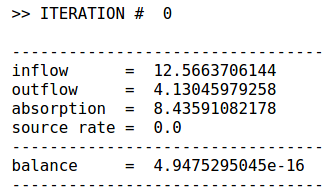
\includegraphics[width=0.35\textwidth]{prob1_table1.png}
\end{figure}

\begin{figure}[!htb]
    \centering
    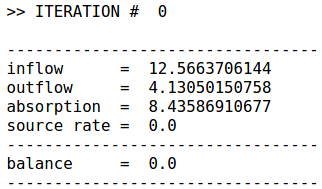
\includegraphics[width=0.35\textwidth]{prob1_table2.png}
\end{figure}

\begin{figure}[!htb]
    \centering
    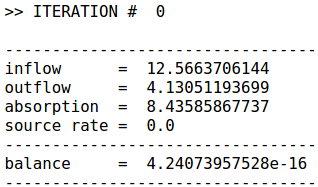
\includegraphics[width=0.35\textwidth]{prob1_table3.png}
\end{figure}

The scalar flux was compared for 50, 100, and 200 spatial cells. As shown in Fig.(1) all three discretization solutions are overlapping and it is difficult to see the difference between each solution. 

\begin{figure}[!htb]
    \centering
    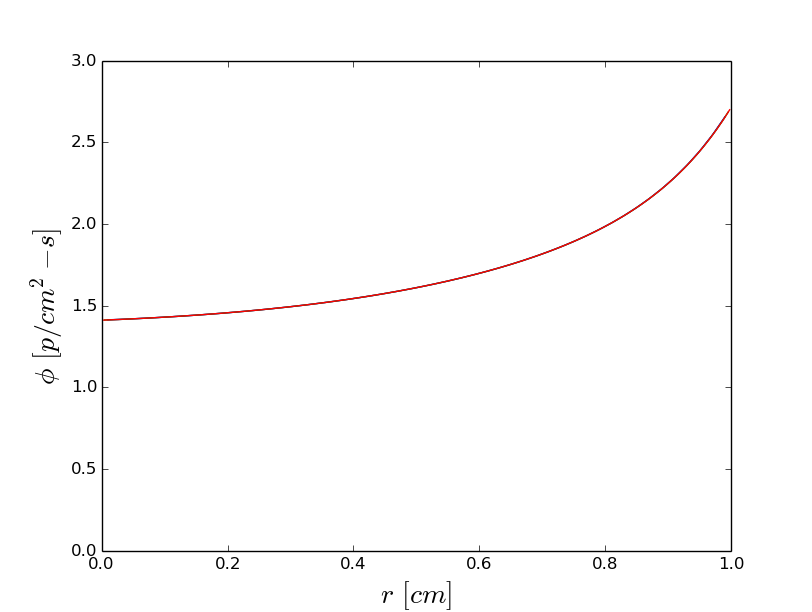
\includegraphics[width=0.6\textwidth]{prob1.png}
    \caption{Scalar flux as a function of $r$ for problem 1.}
    \label{fig:prob1}
\end{figure}

The spatial-covergence order was determined by 
\begin{equation*}
\xi = \frac{\abs{L_{50}-L_{100}}}{\abs{L_{100} - L_{200}}}
\end{equation*}
where $L_k$ denotes the outflow from the outer boundary of the sphere $[p/s]$. The spatial-convergence order was found to be 3.99974 (which is close to the expected value of 4).

\pagebreak

\subsection{Problem 2}

Problem 2 is a sphere of radius = 1 cm, $\sigma_t$ = 3 cm$^{-1}$, and $\sigma_a$ = 1 cm$^{-1}$ with an incident right boundary flux $\phi_o = q_o/\sigma_a$, and a uniformly distributed source of $q_o = 1 [p/cm^3-s]$. We solved for the scalar flux using $S_8$ quadrature and 100 spatial cells with a convergence tolerance of $10^{-4}$. The balance table generated by the $S_N$ code for this problem is shown below. 

\begin{figure}[!htb]
    \centering
    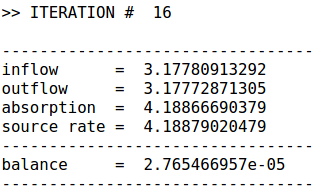
\includegraphics[width=0.35\textwidth]{prob2_table.png}
\end{figure}

We compared the analytical flux $\phi = q/\sigma_s$ to the $S_N$ solution. As shown in Fig.(2) both solution are overlapping, and thus the $S_N$ is behaving as expected.

\begin{figure}[!htb]
    \centering
    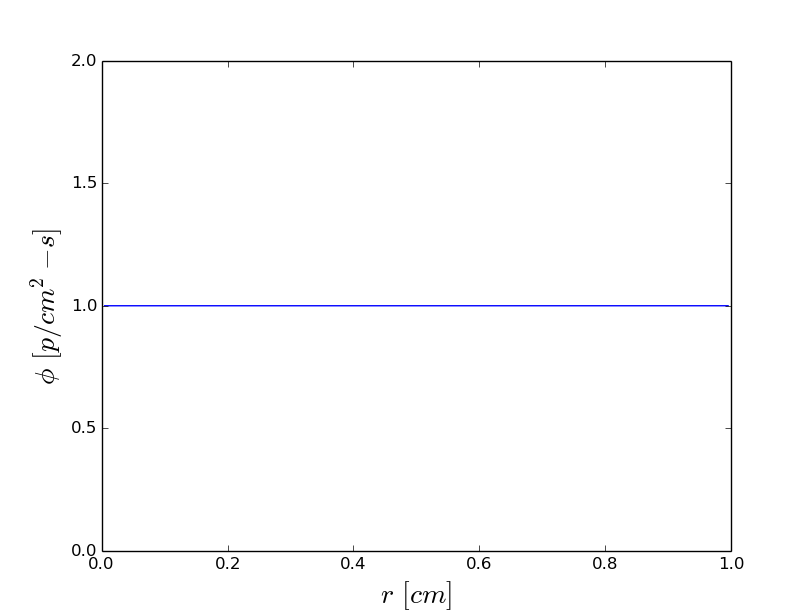
\includegraphics[width=0.6\textwidth]{prob2.png}
    \caption{Scalar flux as a function of $r$ for problem 2.}
    \label{fig:prob2}
\end{figure}

\pagebreak

\subsection{Problem 3}

Problem 3 is a sphere of radius = 1 cm, $\sigma_t$ = 2 cm$^{-1}$, $P_3$ anisotropic scattering with all Legendre coefficients euqal to $\sigma_{s,\ell}$ = 1 cm$^{-1}$ an incoming partial current of 1 $[p/cm^2-s]$. We solved for the scalar flux using $S_4$ quadrature and 100 spatial cells with a convergence tolerance of $10^{-4}$. The balance table for this problem is shown below. 

\begin{figure}[!htb]
    \centering
    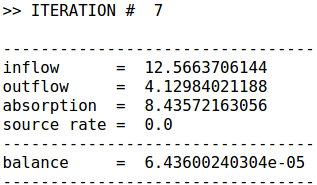
\includegraphics[width=0.35\textwidth]{prob3_table.png}
\end{figure}

In Fig.(3) we compared the flux for problem 1 and problem 3. Both solutions are almost overlapping, thus the solution for problem 3 is behaving as expected. 

\begin{figure}[!htb]
    \centering
    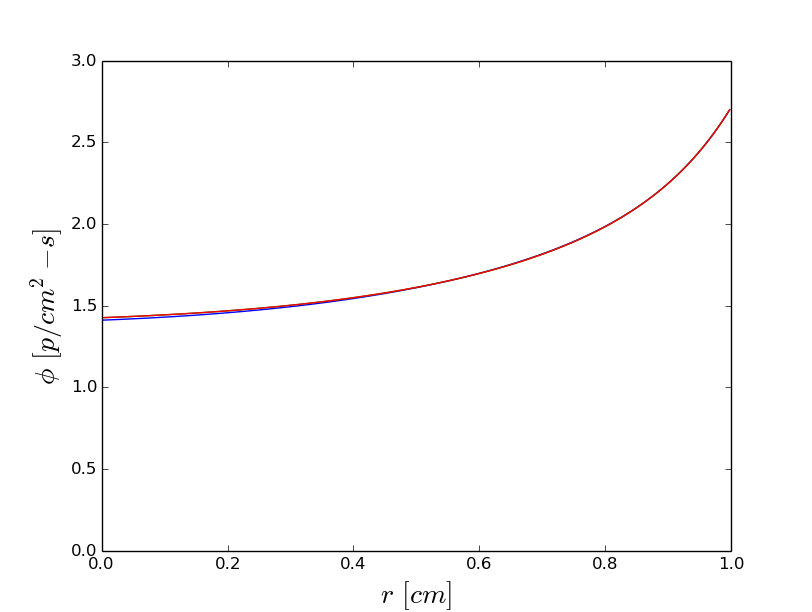
\includegraphics[width=0.6\textwidth]{prob3.png}
    \caption{Scalar flux as a function of $r$ for problem 3.}
    \label{fig:prob3}
\end{figure}

The spatial-convergence order for this problem was 4.00017 (close to the expected value of 4).


\pagebreak

\subsection{Problem 4}

Problem 4 is a sphere of radius = 1 cm, $\sigma_t$ = 30 cm$^{-1}$, and $\sigma_a$ = 0 cm$^{-1}$ with isotropic scattering, a vaccum right boundary condition, and a uniformly distributed source of $q_o = 1 [p/cm^3-s]$. The analytical solution for this problem can be derived using diffusion theory (which is accurate everywhere except at the boundary layer),
\begin{equation*}
- D \nabla^2 \phi + \sigma_a \phi = q_o 
\end{equation*}
\begin{equation*}
- \frac{D}{r^2} \frac{\partial}{\partial r} \Big( r^2 \frac{\partial \phi}{\partial r} \Big) = q_o 
\end{equation*}
\begin{equation*}
\int dr \, \frac{\partial}{\partial r} \Big( r^2 \frac{\partial \phi}{\partial r} \Big) = \int dr \, -\frac{q_o r^2}{D} 
\end{equation*}
\begin{equation*}
 r^2 \frac{\partial \phi}{\partial r} = -\frac{q_o r^3}{3 D} + C_1 
\end{equation*}
\begin{equation*}
\int dr \, \frac{\partial \phi}{\partial r} = \int dr \, -\frac{q_o r}{3 D} + \frac{C_1}{r^2} 
\end{equation*}
\begin{equation*}
\phi = -\frac{q_o r^2}{6 D} - \frac{C_1}{r} + C_2 
\end{equation*}
Now by applying the boundary condition, we can solve for $C_1$ and $C_2$. We know that $\phi$ must be finite at $r=0$, therefore 
\begin{equation*}
C_1 = 0 \: .
\end{equation*}
We can use a Marshak vacuum boundary condition for the right boundary,
\begin{equation*}
\phi(R +2D) = 0
\end{equation*}
\begin{equation*}
-\frac{q_o (R +2D)^2}{6 D} + C_2 = 0
\end{equation*}
\begin{equation*}
\phi = \frac{q}{6 D} \big(R^2 - r^2\big) + \frac{2q}{3} \big(R + D\big)
\end{equation*}

Next, we solved for the scalar flux using $S_8$ quadrature and 100 spatial cells with a convergence tolerance of $10^{-4}$. The balance table for this problem is shown below. 
\begin{figure}[!htb]
    \centering
    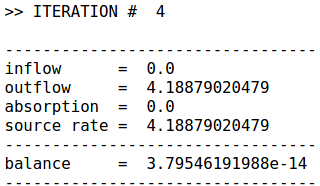
\includegraphics[width=0.35\textwidth]{prob4_table.png}
\end{figure}

We compared the analytic flux to the $S_N$ solution, shown in Fig.(4). Notice that both solutions overlap, thus the solution from the $S_N$ code is behaving as expected. 
\begin{figure}[!htb]
    \centering
    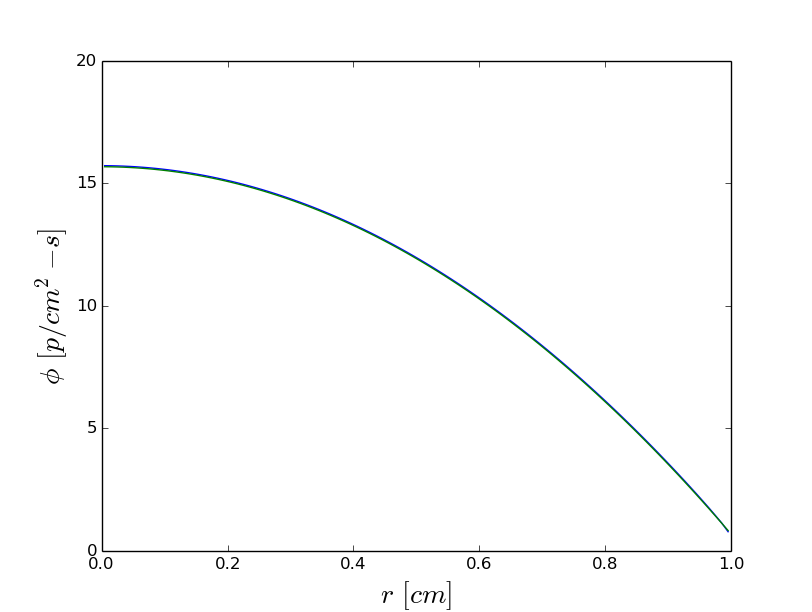
\includegraphics[width=0.6\textwidth]{prob4.png}
    \caption{Scalar flux as a function of $r$ for problem 4.}
    \label{fig:prob4}
\end{figure}




\end{document}

